%************************************************
\chapter{Evaluation}\label{ch:evaluation}
%************************************************

As stated in the introduction, the actual cost of running a virtual machine can be formulated by \autoref{eq:intro}. It is therefore important to develop an accurate model for determining $c_\text{effective}$ and $c_\text{waste}$. Therefore, this section is divided into a number of sub-sections. First, \autoref{sec:model} shows how these cost-values can be computed. Second, the pricing model is computed in \autoref{sec:pricing}.

% I want to answer this question by explaining that the price of a VM can be estimated by a simple formula, for which the data is based on GCE. Additionally, I want to do some research that this price is more or less equivalent across multiple Cloud Providers
%
\subsection{Computing the cost and waste} \label{sec:model}
The effective cost and waste can be monitored per billing time unit (BTU). For most public cloud providers, this BTU is one second. However, it is computationally to intensive to compute the effective cost and waste every second. Instead, an average over a time period of one hour is taken. This leads to the same results as computing it every second. However, the disadvantage is that the desired solution must be up for one hour before a result can be obtained. Additionally, the effective cost are related to the part of the VM that is utilized. Therefore, for a time period of one hour, the effective costs are:

\begin{equation} \label{eq:effective}
c_\text{effective} = p \sum_{i=1}^n u_i
\end{equation}

\noindent
Where $p$ is the price of the actual cost for one hour, and $u_i$ is the average utilization for one hour. This formula can be repeated for expressing the waste in terms of the price for a host and the resource waste:

\begin{equation} \label{eq:waste}
c_\text{waste} = p \sum_{i=1}^n w_i
\end{equation}

\noindent
Where $w_i$ is the average resource waste for one hour. Note that \autoref{eq:effective} and \autoref{eq:waste} both determine the cost for a specific host. In case the deployed system consists of multiple hosts, the values need to be summed. Furthermore, these costs are for a period of one hour. In case the system is deployed for a longer period of time, than this computation needs to be recomputed every hour, and the collected values must be summed. 


\section{Computing the waste distribution} \label{sec:waste_into}
In the sections below, the waste computation will be explained, as well as the decision that have been made that are relevant for computing the waste, given the utlization values for a given host. To rephrase, the research question that will be answered is:

\begin{quote}
    \textbf{Q4: }\textit{What is an effective approach for computing the waste of a Cloud application?}\\
\end{quote}

\noindent
This question can be considered as a mathematical question, as it consists of a fixed set of input variables, and results in a fixed set of output variables. In order to answer this question it is therefore important to determine the properties of the waste distribution before. The next section comes up with three strategies for computing the waste distribution, that all meet the requirements of the properties below. The last section tries to find the optimal approach, by evaluating the approaches against several properties.



\section{Optimal approach} \label{sec:optimal_approach}
\autoref{sec:approaches} describes three different approaches for computing the waste distribution, given the utilization values. This section evaluates the approaches against several properties, and chooses the best approach for the remainder of this chapter.

\subsection{Complexity}
The complexity can be expressed in terms of memory complexity and computational complexity. They are all listed in \autoref{tab:complexity}. The minimal complexity for both memory and computational is $\mathcal{O}(n)$, as a host runs $n$ containers. Approach 2 has a memory complexity of $\mathcal{O}(n)$ as this algorithm only iterates the utilization values as well. Approach 3 has a computational complexity of $\mathcal{O}(n^3)$ as this is necessary for solving a system of linear equations in the worst case. However, \cite{pan1991complexity} explains that there exists several optimization and thus may be usually be done in $\mathcal{O}(n^2)$.\\

\noindent
As approach \ref{sec:proportional} is clearly the worst in terms of memory and computational complexity it can be argued that $n$ is usually not a very large number, as it represents the number of containers for a specific host. According to a survey from 2017 \cite{docker_report}, the median number of containers per host is 10. However, this survey also stated that they have a response with 95 containers per host. In both cases, the waste can be easily computed. On an average machine, computing the waste for for $n = 100$ takes less than 1 millisecond. Given that this needs to be computed only once an hour, all three approaches are sufficient.

\begin{table}[ht]
    \centering
    \begin{tabular}{l|c|c}
        \textbf{Approach} & \textbf{Memory} & \textbf{Computational} \\ \hline
        \ref{sec:equal} & $\mathcal{O}(n)$ & $\mathcal{O}(n)$ \\
        \ref{sec:linear} & $\mathcal{O}(n)$ & $\mathcal{O}(n \log n)$ \\
        \ref{sec:proportional} & $\mathcal{O}(n^2)$ & $\mathcal{O}(n^3)$ \\
    \end{tabular}
    \caption{Memory and Computational complexity for the three different approaches}
    \label{tab:complexity}
\end{table}

\subsection{Data interpretation} \label{sec:data}
As the previous section has shown that the computational and memory complexity is not significant in choosing the best approach, it is interesting to investigate the difference in their results. This section shows the actual values and whether these can be justified. In order to do so, several utilization distributions have been generated and have been listed in \autoref{tab:values}. This table provides two examples with $n = 2$, and two examples with $n = 3$. In the first row, the waste for all three approaches are approximately equivalent. However, in the second row, the waste varies a lot between the different approaches. It doesn't feel natural that, if a container utilizes 4 times more than another container, its corresponding waste is the same. Therefore, the computations from the approach described in \autoref{sec:equal} feel to simplistic.\\

\noindent
In the case of $n = 3$, the table provides two examples. It can be observed that the approach describes in \autoref{sec:linear} returns $0$ if the utilization is too high. However, this might also feel unnatural, as there is the notion that every container might be able to reduce its waste. It also needs to be stated that the approach from \autoref{sec:proportional} might seem incorrect as well, as the it is based on the assumption that every container utilizes and wastes the same amount ($u_i * w_i = c$). Although it is required that $u_i > 0$, it can be close to $0$. This leads to the fact that this container utilizes almost every waste, i.e. $w_i \approx \sum_{i=1}^n w_i$.\\

\noindent
Apart from presenting the data in a table, it is also possible to visualize this in a graph. This visualization can be found in Figure \ref{fig:approaches}. It consists of two examples of utilization distributions, each consisting of two utilization values. This visualization should be interpreted by drawing a vertical line from the utilization values to the waste values. For example, in \autoref{fig:approaches:A}, the utilization values in the left most position are $u_1 = 0.2$ and $u_2 = 0$. This results in $w_1 = w_2 = 0.4$ for approach 1, $w_1 = 0.3, w_2 = 0.5$ for approach 2, and $w_1 = 0, w_2 = 0.8$ for approach 3. Using \autoref{fig:approaches:A}, it can be observed how the waste values change if one utilization value remains constant, while the other utilization value increases. In \autoref{fig:approaches:B} it can be observed how the waste values change while one utilization value increases and another decreases. In this figure, the sum of the utilization values remains constant, while it increases in \autoref{fig:approaches:A}.

\begin{table}
    \centering
    \begin{tabular}{|r|r|r|r|c|r|r|r|r|}
        \hline
        \multicolumn{4}{|c|}{\textbf{Utilization}} & \multirow{2}{*}{\textbf{Approach}} & \multicolumn{4}{|c|}{\textbf{Waste}} \\ 
        $u_1$ & $u_2$ & $u_3$ & $\sum$ & \multirow{2}{*}{} & $w_1$ & $w_2$ & $w_3$ & $\sum$ \\ \hline
        
        \multirow{3}{*}{0.10} & \multirow{3}{*}{0.15} &  & \multirow{3}{*}{0.25} 
        & \ref{sec:equal} & 0.375 & 0.375 & &                            \multirow{3}{*}{0.75} \\
        \multirow{3}{*}{}     & \multirow{3}{*}{}     & & \multirow{3}{*}{}
        & \ref{sec:linear} & 0.4 & 0.35 & & \multirow{3}{*}{} \\
        \multirow{3}{*}{}     & \multirow{3}{*}{}     & & \multirow{3}{*}{}
        & \ref{sec:proportional} & 0.45 & 0.3 & & \multirow{3}{*}{} \\ \hline
        
        \multirow{3}{*}{0.60} & \multirow{3}{*}{0.15} &  & \multirow{3}{*}{0.75} 
        & \ref{sec:equal} & 0.125 & 0.125 & &                            \multirow{3}{*}{0.25} \\
        \multirow{3}{*}{}     & \multirow{3}{*}{}     & & \multirow{3}{*}{}
        & \ref{sec:linear} & 0 & 0.25 & & \multirow{3}{*}{} \\
        \multirow{3}{*}{}     & \multirow{3}{*}{}     & & \multirow{3}{*}{}
        & \ref{sec:proportional} & 0.05 & 0.20 & & \multirow{3}{*}{} \\ \hline
        
        \multirow{3}{*}{0.10} & \multirow{3}{*}{0.35} & \multirow{3}{*}{0.35} & \multirow{3}{*}{0.80} 
        & \ref{sec:equal} & 0.067 & 0.067 & 0.067 & \multirow{3}{*}{0.20} \\
        \multirow{3}{*}{}     & \multirow{3}{*}{}     & \multirow{3}{*}{} & \multirow{3}{*}{}
        & \ref{sec:linear} & 0.20 & 0 & 0 & \multirow{3}{*}{} \\
        \multirow{3}{*}{}     & \multirow{3}{*}{}     & \multirow{3}{*}{} & \multirow{3}{*}{}
        & \ref{sec:proportional} & 0.127 & 0.036 & 0.036 & \multirow{3}{*}{} \\ \hline
        
        \multirow{3}{*}{0.05} & \multirow{3}{*}{0.05} & \multirow{3}{*}{0.45} & \multirow{3}{*}{0.55} 
        & \ref{sec:equal} & 0.15 & 0.15 & 0.15 & \multirow{3}{*}{0.45} \\
        \multirow{3}{*}{}     & \multirow{3}{*}{}     & \multirow{3}{*}{} & \multirow{3}{*}{}
        & \ref{sec:linear} & 0.225 & 0.225 & 0 & \multirow{3}{*}{} \\
        \multirow{3}{*}{}     & \multirow{3}{*}{}     & \multirow{3}{*}{} & \multirow{3}{*}{}
        & \ref{sec:proportional} & 0.213 & 0.213 & 0.023 & \multirow{3}{*}{} \\ \hline
        
    \end{tabular}
    \caption{Several utilization values and the waste values that are computed using the three approaches}
    \label{tab:values}
\end{table}


\begin{figure}
    \subfloat[Example 1]{%
        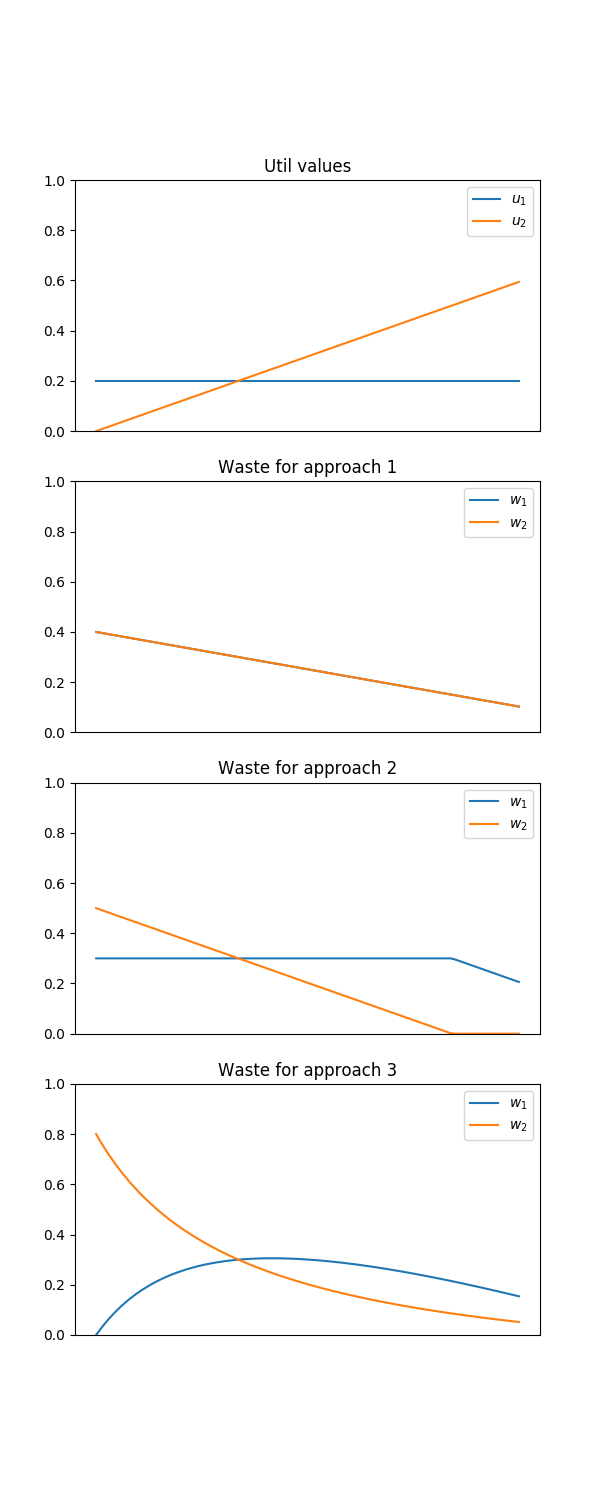
\includegraphics[width=6cm]{gfx/exampleA.png}%
        \label{fig:approaches:A}%
    }\qquad
    \subfloat[Example 2]{%
        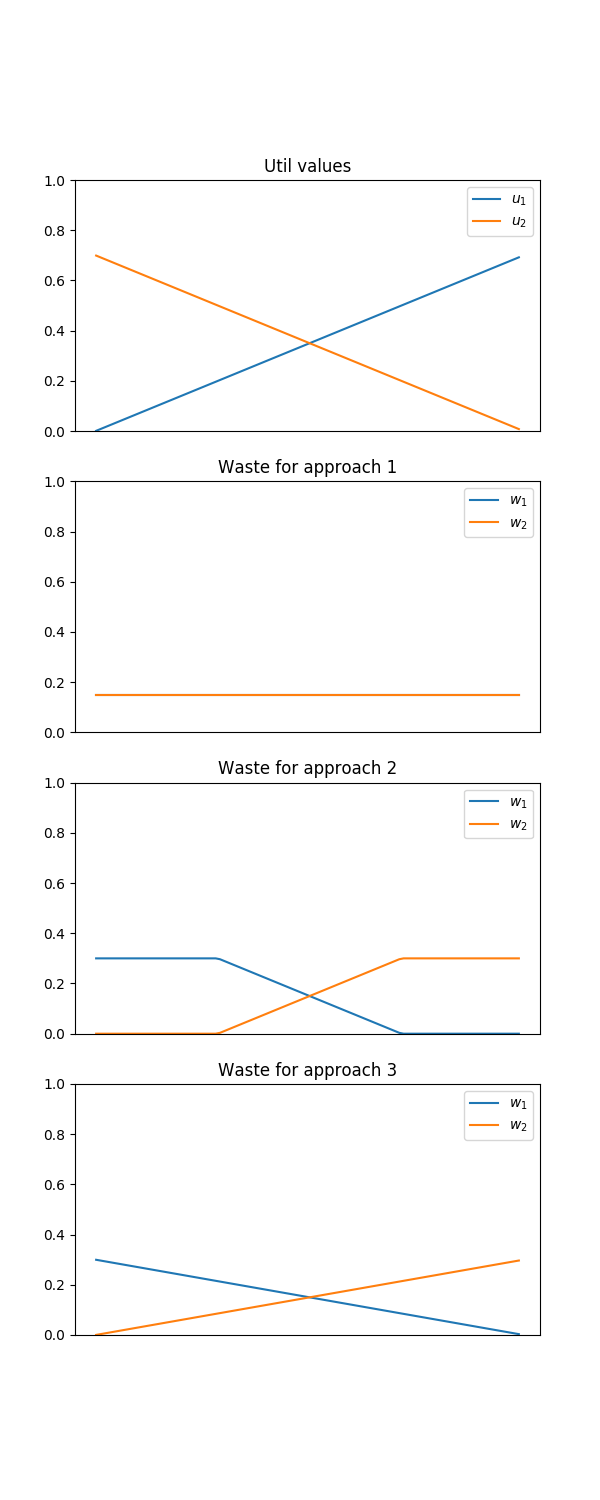
\includegraphics[width=6cm]{gfx/exampleB.png}%
        \label{fig:approaches:B}%
    }
    \caption{Two utilization values and their corresponding waste distribution}
    \label{fig:approaches}
\end{figure}


\section{Conclusion} \label{sec:conclusion4}
One of the properties of the utilization values (as stated in \autoref{sec:utilization}) is that $u_i > 0$ for all $i$. However, while deploying the system, it turned out that the utilization of a certain container was zero. In the first two approaches (\autoref{sec:equal} and \autoref{sec:linear}), this is not a problem. However, this is a problem for the last approach (\autoref{sec:proportional}). An example can be seen for $n = 3$ with $u_1 = 0.3, u_2 = 0, u_3 = 0.2$. This results in the waste values: $w_1 = 0, w_2 = 0.5, w_3 = 0$. Therefore, if $u_1 = 0$, then $w_i = 1 - u$.\\

\noindent
In case there are two containers that have a zero utilization, than the waste cannot be computed for the third approach. This is due to the fact that the matrix $A_n$ does not have a full rank anymore (as two rows are the same). This problem can be avoided by adding a small utilization value $\Delta$ to the $u_i$-values that are $0$. This value can then be removed from the corresponding $w_i$ value, to ensure that property 1 still holds. However, as explained in \autoref{sec:data}, the corresponding $w_i$ will be close to $\sum_{j=1}^n w_j$ and will lead to abnormal results. This leads to the conclusion that only the approach from \autoref{sec:linear} is sufficient for the implementation. Thus, Algorithm \ref{alg:linear} will be used to compute the waste values given the utilization values.